\subsection{Reasoning through Transimpedance Logarithmic Photoreceptor}

This is common exam question!

\begin{figure}[H]
    \centering
    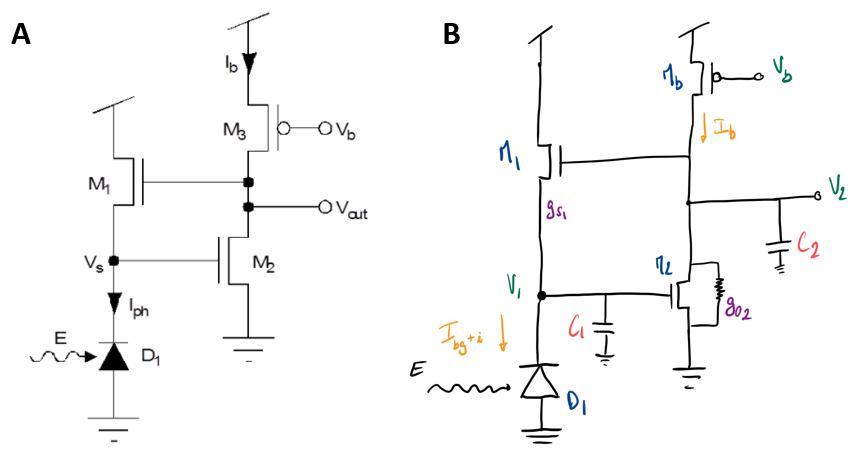
\includegraphics[width=1\linewidth]{../../Figures/Transimpedance_Log_Photoreceptor_Full.PNG}
    \caption{A) Basic Transimpedance Logarithmic Photoreceptor diagram. We only need this for DC response. B) Transimpedance Logarithmic Photoreceptor which considers the parasitic capacitance and conductance, which need to be considered for the time frequency response. We will be using naming conventions of B) in our analysis. Adapted from Lecture notes.}
    \label{fig:Transimpedance_Log_Photoreceptor_Full}
\end{figure}


\begin{enumerate}
    \item Circuit follows the same logic, except that instead of $M_1$ having a fixed gate voltage as in the source follower, we have some kind of inverting amplifier setting that controls it. 
    \item Photodiode still acts as a constant current sink as in the previous source follower arrangement.
    \item $M_3$ is a saturated pFET which draws a constant current $I_b$. 
    \item Similarly to before, $V_1$, gate voltage of $M_2$, must be at a value that matches the current $I_b$ flowing in the right branch. It follows that $V_1$ must match $V_b$. That is, $V_{dd} - V_b = V_1 - 0$.
    \item $V_2$, gate voltage of $M_1$ must provide a $V_{gs}$ to $M_1$ that will match $I_{bg} + i$. Note that $V_{gs}$ of $M_b$ is $V_2 - V_1$
    \item \textbf{Important:} A popular exam question to take some values for a starting voltage point and reason you way through the rest. This is particularly true where we can reason through the DC output of this circuit: 
    \begin{enumerate}
        \item Let's for example assume that $V_1 = 0.7V$
        \item We thus from 1. need to have $V_{dd} - V_b = 0.7V$.
        \item Let's assume that we have a saturated transistor instead of a photodiode. This allows us to have a voltage to reason with rather than current, though both effectively do the same thing: provide constant current from constant input. This is just for the sake of the analysis because we can now choose a gate voltage for this transistor $M_0$ that we call $V_g_0$.
        \item If we take gate voltage of this transistor to be $V_g_0 = 0.4 V$, then it follows from 2. that $V_2 - V_1 = 0.4 v$. 
        \item We thus have value of $V_2 = 1.1 V$! 
    \end{enumerate}
    \item The DC response of this circuit is: 
    \begin{equation}
        V_2 = k^{-1}(V_1 + U_t\mathrm{log}(\frac{I_ph}{I_0})
    \end{equation}
    Note that this doesn't consider the parasitic capacitance and conductance as we're doing the DC output. 
    \item \textbf{Summary}: This circuit is an improvement of the previous one, where we enhance the response speed by adding a high-gain negative feedback lop from the source to the gate of the MOSFET in the previous source follower configuration. The voltage output signal then appears at the gate of the MOSFET, while the source and therefore the voltage across the photodiode is practically clamped.
\end{enumerate}

\subsubsection{Time domain response of transimpedance logarithmic Photoreceptor}

\begin{enumerate}
    \item From the circuit we can get the following differential equations for $V_1$ and $V_2$:
    \begin{equation}
        C_1\dot{V_1} = I_0 e^{\frac{\kappa V_2 - V_1}{U_T}} - I_{ph}
    \end{equation}
    \begin{equation}
        C_2\dot{V_2} = I_b - g_{o2}V_2 - I_0 e^{\frac{\kappa V_1}{U_T}} 
    \end{equation}
    
    \item In the small signal regime, we can simplify this to:
    \begin{equation}
        C_1\dot{v_1} = g_{m1} v_2 - g_{s1} v_1 - i
    \end{equation}
    \begin{equation}
        C_2\dot{v_2} = -g_{o2}v_2 - g_{m2}v_1
    \end{equation}
    
    with $g_{s1} = \frac{-I_{ph}}{U_T}$, $g_{m1} = \frac{\kappa I_{ph}}{U_T}$, $g_{o2} = \frac{I_b}{V_e}$, $g_{m2} = \frac{\kappa I_b}{U_T}$
    
    Note that we also neglected $I_b$ here, as it is constant and we are interested in the small changes only.
    
    \item By defining the time constants $\tau_1 = \frac{C_1}{g_{s1}}$ and $\tau_2 = \frac{C_2}{g_{o2}}$ and remembering how to use Laplace transform to solve linear differential equations (just replace the derivative with multiplication by s), we can rewrite this to:
    \begin{equation}
        (\tau_1 s + 1) v_1= \frac{g_{m1}}{g_{s1}} v_2 - \frac{i}{g_{s1}}
    \end{equation}
    \begin{equation}
       (\tau_2 s + 1) v_2 = - \frac{g_{m2}}{g_{o2}}v_1 = -A v_1
    \end{equation}
    where $A$ is the gain of the output transistor by definition.
    
    \item Solving this system of polynomial equations, we get:
    \begin{equation}
        v_2 = \frac{-\frac{A}{g_{s1}}}{\tau_1 \tau_2 s^2 + (\tau_1 + \tau_2) s + 1 + kA}
    \end{equation}
    
    
\end{enumerate}

  